% Budget: 1.70 pp (AGENT) / 1.25 pp (ICRITO).
% Sources: paper/generated/verdicts.md; numbers.tex; posthoc.tex; contrasts_faulty_tex.tex (T4);
% crash_matrix.tex (T3); figs/f4_false_closure.pdf; docs/POSTHOC.md; docs/CHANGELOG_RESEARCH.md.
% Every number is a macro. Post-hoc results (PH2-PH8) are labelled in the text.
\section{Results}\label{sec:results}

All pre-registered verdicts follow from the frozen decision rules: H1, H2, H4, H5 and C1 are \VerdictHOne, and H3 is \VerdictHThree.

\subsection{Acknowledgment-trust closes falsely (H1)}\label{sec:results:h1}
P3 reports false closures in \NFaultyCellsAckFC{} of the \NFaultyCells{} faulty primary cells (Fig.~\ref{fig:falseclosure}). At low faults, \FCAckLow{} of its \FCClosedCancelledAckLow{} \textsc{closed\_cancelled} reports are false, a share of \FCShareAckLow{} (Wilson \lit{95\%} interval \FCShareLoAckLow--\FCShareHiAckLow); at high faults the share rises to \FCShareAckHigh{} (\FCShareLoAckHigh--\FCShareHiAckHigh). P1 and P2 also close falsely at both fault levels, and the pre-registered criterion for a negligible false-closure rate is \VerdictNegligibleFalseClosure. Each of these closures is a payment that a dashboard would show as stopped while the merchant captured it. P0 and P4--P6 report no false closure in any holdout run. That half of H1 holds by construction (Proposition~\ref{prop:evidence}); it verifies the implementation, and the checker's mutation tests show that a false closure would not go unseen.

P3 lacks the sweep and late cancellation that P4--P6 have (Section~\ref{sec:runbooks}). Switching late cancellation off for P4--P6 at jitter twice the primary value changes their mean loss by between $\AblLateCancelVerifyNoneTightJUniformSix$ and $\AblLateCancelVerifyHighNormalJUniformSix$ per run, small against the H2 effects below.

\begin{figure}[t]
  \centering
  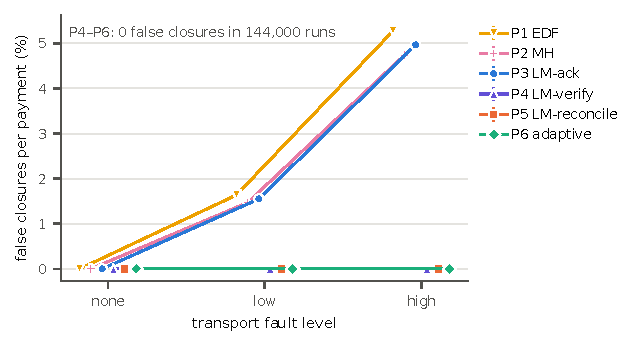
\includegraphics[width=0.92\columnwidth]{f4_false_closure}
  \caption{False closures per payment by fault level, primary grid. P0 and P4--P6 report none in any of their runs.}
  \label{fig:falseclosure}
\end{figure}

% Generated by analysis/report.py. Do not edit by hand.
% Holm family: every row of contrasts_primary.csv. The Holm CI is the percentile CI at level 1 - alpha/(m - rank + 1) (analysis/stats.py).
\begin{table}[t]
\centering
\scriptsize
\setlength{\tabcolsep}{4pt}
\caption{Paired loss differences in the 16 faulty primary cells (fault/slack/$k$/$n$): mean and CI at each contrast's Holm level. $^\dagger$\,Holm-adjusted $p \le 0.05$.}
\label{tab:contrasts-faulty}
\begin{tabular}{lrr}
\toprule
Cell & P4$-$P3 $\Delta$ [Holm CI] & P5$-$P3 $\Delta$ [Holm CI] \\
\midrule
low/tight/1/8 & 50.1 [22.0, 80.7]$^\dagger$ & $-$8.9 [$-$18.7, $-$1.0]$^\dagger$ \\
low/tight/1/32 & 158.7 [108.9, 211.3]$^\dagger$ & $-$6.5 [$-$15.8, 0.7] \\
low/tight/4/8 & $-$25.6 [$-$45.8, $-$7.0]$^\dagger$ & $-$35.9 [$-$57.6, $-$13.9]$^\dagger$ \\
low/tight/4/32 & 145.9 [84.9, 207.1]$^\dagger$ & $-$33.0 [$-$52.2, $-$15.3]$^\dagger$ \\
low/normal/1/8 & 48.5 [16.8, 85.0]$^\dagger$ & $-$8.6 [$-$19.6, 0.6] \\
low/normal/1/32 & 238.9 [175.0, 304.5]$^\dagger$ & $-$4.6 [$-$12.6, 1.8] \\
low/normal/4/8 & $-$43.2 [$-$67.9, $-$20.1]$^\dagger$ & $-$46.0 [$-$71.1, $-$22.1]$^\dagger$ \\
low/normal/4/32 & 113.3 [47.4, 180.1]$^\dagger$ & $-$39.9 [$-$61.0, $-$20.5]$^\dagger$ \\
high/tight/1/8 & 155.8 [107.7, 201.5]$^\dagger$ & $-$15.4 [$-$31.0, $-$1.8]$^\dagger$ \\
high/tight/1/32 & 427.9 [346.4, 515.1]$^\dagger$ & $-$13.2 [$-$25.3, $-$2.1]$^\dagger$ \\
high/tight/4/8 & $-$70.4 [$-$101.6, $-$38.6]$^\dagger$ & $-$117.0 [$-$154.8, $-$81.1]$^\dagger$ \\
high/tight/4/32 & 383.4 [302.3, 470.2]$^\dagger$ & $-$68.0 [$-$98.6, $-$39.0]$^\dagger$ \\
high/normal/1/8 & 165.9 [110.4, 218.9]$^\dagger$ & $-$24.5 [$-$43.4, $-$8.5]$^\dagger$ \\
high/normal/1/32 & 605.3 [515.7, 704.1]$^\dagger$ & $-$17.1 [$-$30.0, $-$5.8]$^\dagger$ \\
high/normal/4/8 & $-$143.7 [$-$185.2, $-$101.9]$^\dagger$ & $-$172.3 [$-$217.7, $-$129.8]$^\dagger$ \\
high/normal/4/32 & 428.5 [330.0, 522.0]$^\dagger$ & $-$86.4 [$-$116.9, $-$56.8]$^\dagger$ \\
\bottomrule
\end{tabular}
\end{table}


\subsection{The cost of assurance depends on when it is paid (H2)}\label{sec:results:h2}
Table~\ref{tab:contrasts-faulty} lists both pre-registered contrasts for the faulty cells. Verifying each timeout before the next cancel is expensive when workers are scarce. At tight slack, $k = 1$ and $n = 32$, P4 loses $\DiffVerifyAckLowTightKOneNThirtyTwo$ more than P3 at low faults and $\DiffVerifyAckHighTightKOneNThirtyTwo$ more at high faults, with Holm-level lower bounds of $\HTwoMinHolmLoLow$ and $\HTwoMinHolmLoHigh$; H2 is supported. Across the Holm family, P4 is significantly worse than P3 in \NHolmHigherVerifyAck{} cells and better in \NHolmLowerVerifyAck.

Reconcile-after behaves differently. P5 is never significantly worse than P3 (\NHolmHigherReconcileAck{} cells) and is significantly better in \NHolmLowerReconcileAck{} cells, all of them faulty, while reporting no false closure. Its timed-out cancels wait in a queue instead of blocking a worker, and a replay doubles as a status probe, so the evidence arrives late but costs little. In this model, then, assurance costs loss when it is synchronous and is close to free when it is deferred.

Four post-hoc analyses qualify this result.
\emph{Timeout cost (PH3, development seeds).} The simulator returns a timeout as fast as a reply. When timeouts take $m$ times as long, P4$-$P3 at H2's cells falls from $\PHThreeVerifyAckLowMOne$ to $\PHThreeVerifyAckLowMFour$ (low) and from $\PHThreeVerifyAckHighMOne$ to $\PHThreeVerifyAckHighMFour$ (high) as $m$ grows from one to four, because P3 also waits out its own timeouts. P5's advantage shrinks with it: at $k = 1$, $n = 32$, the interval of P5$-$P3 lies entirely below zero in \PHThreeReconcileAckKOneNThirtyTwoMOneCellsBelow{} of \PHThreeReconcileAckKOneNThirtyTwoMOneCells{} faulty cells at $m$ of one and in \PHThreeReconcileAckKOneNThirtyTwoMFourCellsBelow{} at $m$ of four.
\emph{Simultaneous intervals (PH6).} With Bonferroni-level intervals over the family of \PHSixFamilySize, the H2 lower bounds remain $\PHSixBonfLoVerifyAckLow$ and $\PHSixBonfLoVerifyAckHigh$.
\emph{Where P4 wins (PH5).} The \PHFiveCellsVerifyBetter{} cells where P4 beats P3 are the faulty cells at $k = 4$, $n = 8$. There, re-sending a timed-out cancel recovers between \PHFiveResendShareHighNormalKFourNEight{} and \PHFiveResendShareLowTightKFourNEight{} of the difference (above full when other effects push the other way): retrying is free when workers are idle.
\emph{Retrying without evidence (PH2, development seeds).} A variant of P3 that retries every timeout but still trusts acknowledgments (P3b) lowers the false-closure share to \PHTwoFCShareAckRetryLow{} (low) and \PHTwoFCShareAckRetryHigh{} (high) from P3's \PHTwoFCShareAckLow{} and \PHTwoFCShareAckHigh{} on the same seeds. P5 is below P3b in \PHTwoReconcileAckRetryCellsBelow{} of \PHTwoReconcileAckRetryCells{} faulty cells and above it in none. Retrying reduces false closures; only evidence removes them.

\subsection{The shared scheduler at \texorpdfstring{\lit{$k > 1$}}{multiple workers} (PH8, post hoc)}\label{sec:results:sched}
All contrasts above hold the scheduler fixed. Absolute loss does not: at $k = 4$, $n = 32$, the mean of P2$-$P3 ranges from $\PHEightMhAckMinAllKFourNThirtyTwo$ to $\PHEightMhAckMaxAllKFourNThirtyTwo$ per run across fault and slack levels, faultless cells included, and P2$-$P5 from $\PHEightMhReconcileMinAllKFourNThirtyTwo$ to $\PHEightMhReconcileMaxAllKFourNThirtyTwo$: P2's weighted Moore heuristic has the lower loss. At $k = 4$, $n = 8$ the difference to P3 lies between $\PHEightMhAckMinAllKFourNEight$ and $\PHEightMhAckMaxAllKFourNEight$. The lowest-loss runbook in those larger cells is therefore an ACK-trust one, and it still closes falsely (\FCMhHigh{} false closures over the high-fault cells). Lawler--Moore is exact only at $k = 1$, and an evidence-bounded runbook on a stronger multi-worker scheduler was not part of the study.

\subsection{Adaptive re-planning and the control (H3, H4)}\label{sec:results:h3h4}
Re-planning at every free-worker event adds nothing measurable to reconcile-after. At $k = 1$, P6 and P5 differ in loss on \HThreeNonzeroSeedsKOne{} of \HThreeSeedsKOne{} seeds. At $k = 4$ they differ on \HThreeNonzeroSeedsKFour{} of \HThreeSeedsKFour{} seeds, yet none of the \HThreeCellsKFour{} intervals excludes zero, so H3 is not supported, as development data had predicted. The negative control behaves as a sanity check should: with unlimited workers, no faults and no jitter, P3--P6 incur equal loss on \NegCtrlSeedsEqual{} of \NegCtrlSeeds{} seeds, since every runbook sends every planned cancel at once and every call succeeds.

% Generated by analysis/report.py. Do not edit by hand.
% Rows sum each policy's crash-matrix cells over all their runs, crashed or not.
% Crashed (min): crashed runs, and in parentheses the fewest crashed runs in one cell.
% FC/FE/Dup: false closures, false exposures, duplicate effects; Inv: runs with a failed invariant.
% A cell holds with FC = FE = Dup = Inv = 0 and at least 100 crashed runs (H5).
\begin{table}[t]
\centering
\scriptsize
\setlength{\tabcolsep}{4pt}
\caption{Crash matrix (H5), summed over each policy's cells. P3's false closures are measurements; P3 is not part of H5.}
\label{tab:crash-matrix}
\begin{tabular}{lrrrr}
\toprule
Policy & Cells held & Crashed (min) & FC & FE/Dup/Inv \\
\midrule
P3 & -- & 50{,}808 (2{,}808) & 21{,}644 & 0/0/0 \\
P4 & 13/13 & 114{,}500 (3{,}803) & 0 & 0/0/0 \\
P5 & 13/13 & 111{,}977 (3{,}170) & 0 & 0/0/0 \\
P6 & 13/13 & 111{,}769 (3{,}126) & 0 & 0/0/0 \\
\bottomrule
\end{tabular}
\end{table}


\subsection{Safe resumption of remediation (H5)}\label{sec:results:h5}
Table~\ref{tab:crash-matrix} summarizes the crash matrix. For P4--P6, all \HfiveCellsHold{} (cell, runbook) pairs hold: across \num{\HfiveCrashedRuns} crashed runs, with at least \num{\HfiveMinCrashed} per pair, the checker finds \HfiveFalseClosures{} false closures, \HfiveFalseExposures{} false exposures and \HfiveDuplicateEffects{} duplicate effects, and no failed invariant. The combination of a fixed cancel key, processor-side idempotency and the write-ahead journal therefore survives one crash per episode at every call point we instrumented. P3, which re-sends orphaned intents and trusts the reply, keeps closing falsely after a restart.

The claim covers one crash per episode. In a post-hoc run on development seeds with two crashes per episode (PH7), \PHSevenPairsHold{} of \PHSevenPairs{} pairs hold over \PHSevenCrashedTwice{} doubly crashed runs. The same exercise exposed a defect in the frozen P3: two crashes before one cancel's result is journaled leave two orphaned intents, and its outbox recovery fails. The holdout matrix crashes at most once per run, so no frozen result is affected; we leave P3 unchanged because it is the frozen baseline.
